\documentclass[12pt]{article}

\usepackage{sbc-template}
\usepackage{graphicx,url}
\usepackage[latin1]{inputenc}
\usepackage{prooftree}
\usepackage{float}
\usepackage{framed}
\usepackage{amsmath}
\usepackage{mathtools}
\usepackage{listings}
\usepackage{color}

\definecolor{dkgreen}{rgb}{0,0.6,0}
\definecolor{gray}{rgb}{0.5,0.5,0.5}
\definecolor{mauve}{rgb}{0.58,0,0.82}

\lstset{frame=tb,
  aboveskip=3mm,
  belowskip=3mm,
  showstringspaces=false,
  columns=flexible,
  basicstyle={\small\ttfamily},
  numbers=none,
  numberstyle=\tiny\color{gray},
  keywordstyle=\color{blue},
  commentstyle=\color{dkgreen},
  stringstyle=\color{mauve},
  breaklines=true,
  breakatwhitespace=true,
  language=ml,
  tabsize=3
}

\sloppy

\title{M�todos Formais\\ Trabalho I}

\author{Matthias Oliveira de Nunes}

\address{Faculdade de Inform�tica -- Pontif�cia Universidade Cat�lica do Rio
        Grande do Sul (PUCRS)\\
        Av. Ipiranga, 6681 Partenon Porto Alegre/RS CEP: 90619-900 -- Brazil
\email{matthiasnunes@gmail.com}}

\begin{document} 

\maketitle

\begin{abstract}
  This meta-paper describes the first assingment of the Formal Methods course,
  on which we define four primitive recursive functions, for the generic binary
  tree datatype, and prove two theorems.
\end{abstract}
     
\begin{resumo}
  Este meta-artigo descreve o primeiro trabalho da cadeira de M�todos formais,
  onde definimos quatro fun��es primitivas recursivas, para o tipo de dado
  �rvore gen�rica, e provamos dois teoremas.
\end{resumo}

\section{Introdu��o} \label{sec:intro}

Dentro do escopo da disciplina de M�todos Formais, 


\section{Defini��es e Teoremas} \label{sec:def}

Como explicado anteriormente, um conjunto indutivo possui \emph{construtores}.
Isso � relevante pois mostraremos agora a defini��o de dois tipos de dados:
\emph{Listas Gen�ricas} e \emph{�rvores Bin�rias Gen�ricas}.

\subsection{Listas Gen�ricas}
\label{sub:Lista}

Foram definidos dois construtores para uma \emph{Lista Gen�rica}, 


uahfuaeh fuaehf auehf auehfu aehfuae hfuhae fuhaeuf aeufh aeufh aeufhaeuhf uaehf
aeufh aeufh aeuhf aeufhuaeh fuaehf uaefh uaehf uaehfu aehf aeufhae ufhuaeh
fuaehf uaeh fuae hfuaeh f

$$
\begin{prooftree}
\justifies
  nil \in List(\tau)
\proofdotseparation=1.2ex
\thickness=0.08em
\using
  ListEmpty
\end{prooftree}
$$

$$
\begin{prooftree}
  e \in \tau
  \;\;\;
  L \in List(\tau)
\justifies
  cons \;  e \; L
\proofdotseparation=1.2ex
\thickness=0.08em
\using
  ListCons
\end{prooftree}
$$

\begin{center}
  \begin{framed}
    \begin{prooftree}
      \[
      \proofdotseparation=1.2ex
      \proofdotnumber=4
      \leadsto
        P \; nil
      \]
      \[
        e_0 : \tau, l_0 : List(\tau), P(l_0)
      \proofdotseparation=1.2ex
      \proofdotnumber=4
      \leadsto
      P \; (cons \; e_0 \; L_0)
      \]
      (e_0, l_0 \; arbitr\acute{a}rios)
      \justifies
        \forall l : List(\tau). \; P \; l
      \proofdotseparation=1.2ex
      \thickness=0.08em
      \using
        IndList
    \end{prooftree}
  \end{framed}
\end{center}

\begin{align*}
  cat& \; : \; List(\tau) \rightarrow List(\tau) \rightarrow List(\tau) & \\
  cat& \; nil \; l = l & \text{cat01}\\
  cat& \; (cons \; e \; l_1) \; l_2 = cons \; e \; (cat \; l_1 \; l_2) &
  \text{cat02}\\
\end{align*}

\begin{align*}
  rev& \; : \; List(\tau) \rightarrow List(\tau) & \\
  rev& \; nil = nil & \text{rev01} \\
  rev& \; (cons \; e \; l) = cat \; (rev \; l) (cons \; e \; nil) & \text{rev02}
  \\
\end{align*}

\subsection{�rvores Bin�rias Gen�ricas}
\label{sub:Arvore}

$$
\begin{prooftree}
\justifies
  leaf \in BTree(\tau)
\proofdotseparation=1.2ex
\thickness=0.08em
\using
  BTreeEmpty
\end{prooftree}
$$

$$
\begin{prooftree}
  x \in \tau
  \;\;\;
  L \in BTree(\tau)
  \;\;\;
  R \in BTree(\tau)
\justifies
  br \;  x \; L \; R
\proofdotseparation=1.2ex
\thickness=0.08em
\using
  BTreeBranch
\end{prooftree}
$$

\begin{center}
  \begin{framed}
    \begin{prooftree}
      \[
      \proofdotseparation=1.2ex
      \proofdotnumber=4
      \leadsto
        P \; leaf
      \]
      \[
        x_0 : \tau, lt_0, rt_0 : BTree(\tau), P(lt_0), P(rt_0)
      \proofdotseparation=1.2ex
      \proofdotnumber=4
      \leadsto
      P \; (x_0, lt_0, rt_0)
      \]
      (x_0, lt_0, rt_0 \; arbitr\acute{a}rios)
      \justifies
        \forall t : BTree(\tau). \; P \; t
      \proofdotseparation=1.2ex
      \thickness=0.08em
      \using
        IndBTree
    \end{prooftree}
  \end{framed}
\end{center}


\begin{align*}
  in& \; : \; BTree(\tau) \rightarrow List(\tau) & \\
  in& \; leaf = nil & \text{in01} \\
  in& \; (br \; x \; l \; r) = cat \; (in \; l) \; (cons \; x \; (in \; r)) &
  \text{in02} \\
\end{align*}


\begin{align*}
  pos& \; : \; BTree(\tau) \rightarrow List(\tau) & \\
  pos& \; leaf = nil & \text{pos01} \\
  pos& \; (br \; x \; l \; r) = cat \; (pos \; l) \; (cat \; (pos \; r) \;(cons
  \; x \; nil)) & \text{pos02} \\
\end{align*}

\begin{align*}
  pre& \; : \; BTree(\tau) \rightarrow List(\tau) & \\
  pre& \; leaf = nil & \text{pre01} \\
  pre& \; (br \; x \; l \; r) = cons \; x \; (cat \; (pre \; l) \; (pre \; r)) &
  \text{pre02} \\
\end{align*}

\begin{align*}
  ref& \; : \; BTree(\tau) \rightarrow BTree(\tau) & \\
  ref& \; leaf = leaf & \text{ref01} \\
  ref& \; (br \; x \; l \; r) = br \; x \; (ref \; l) \; (ref \; r) &
  \text{ref02} \\
\end{align*}

\section{Provas}

\subsection{Prova do Teorema 1}
\label{sub:pth01}

\begin{align*}
  P &\doteq \forall x:BTree(\tau). \; pos \; (ref \; x) = rev \; (pre \; x) \\
  P(n) &\doteq pos \; (ref \; n) = rev \; (pre \; n) \\
\end{align*}

\emph{Prova do caso base:}

Temos que mostrar que \[pos \; (ref \; leaf) = rev \; (pre \; leaf)\] ent�o �
suficiente provar que

\begin{align*}
  pos \; (ref \; leaf) &= pos \; leaf & \text{by re01} \\
  ... &= nil & \text{by pos01} \\
  ... &= rev \; nil & \text{by rev01} \\
  ... &= rev \; (pre \; leaf) & \text{by pre01} \\
  qed & & \\
\end{align*}

\emph{Prova do caso indutivo:}

Sejam $x_0:\tau, l:BTree(\tau), r:BTree(\tau)$ vari�veis arbitr�rias. Assumimos
como hip�teses de indu��o

\begin{align*}
  pos \; (ref \; l) &= rev \; (pre \; l) & \text{IH1} \\
  pos \; (ref \; r) &= rev \; (pre \; r) & \text{IH2} \\
\end{align*}

Com isso � suficiente demonstrar que

\begin{align*}
  pos \; (ref \; (br \; x \; l \; r)) &= pos \; (br \; x \; (ref \; r) \; (ref
  \; l)) & \text{by re02} \\
  ... &= cat \; (pos \; (ref \; r)) \; (cat \; (pos \; (ref \; l)) \; (cons \; x
  \; nil)) & \text{by IH2} \\
  ... &= cat \; (rev \; (pre \; r)) \; (cat \; (pos \; (ref \; l)) \; (cons \; x
  \; nil)) & \text{by IH1} \\
  ... &= cat \; (rev \; (pre \; r)) \; (cat \; (rev \; (pre \; l)) \; (cons \; x
  \; nil)) & \text{by catAssociativity} \\
  ... &= cat \; (cat \; (rev \; (pre \; r)) \; (rev \; (pre \; l))) \; (cons \;
  x \; nil) & \text{by thRev} \\
  qed & & \\
\end{align*}

\subsection{Prova do Teorema 2}
\label{sub:pth02}

\begin{align*}
  P &\doteq \forall x:BTree(\tau). \; rev \; (in \; (ref \; x)) = in \; x \\
  P(n) &\doteq rev \; (in \; (ref \; n)) = in \; n \\
\end{align*}

\emph{Prova do caso base:}

Temos que mostrar que \[rev \; (in \; (ref \; leaf)) = in \; leaf\] ent�o �
suficiente provar que

\begin{align*}
  rev \; (in \; (ref \; leaf)) &= rev \; (in \; leaf) & \text{by re01} \\
  ... &= rev \; nil & \text{by in01} \\
  ... &= nil & \text{by rev01} \\
  ... &= in \; leaf &  \text{by in01} \\
  qed & & \\
\end{align*}

%theorem th02: "rev (in (ref x)) = in x"
  %proof (induction x)
    %show "rev (in (ref leaf)) = in leaf"
      %proof -
        %have "rev (in (ref leaf)) = rev (in leaf)" by (simp only: re01)
        %also have "... = rev nil" by (simp only: in01)
        %also have "... = nil" by (simp only: rev01)
        %also have "... = in leaf" by (simp only: in01)
        %finally show ?thesis by this
      %qed
      %next
        %fix x::'a and l::"'a btree" and r::"'a btree"
        %assume IH1: "rev (in (ref l)) = in l"
        %assume IH2: "rev (in (ref r)) = in r"
        %show "rev (in (ref (br x l r))) = in (br x l r)"
          %proof -
            %have "rev (in (ref (br x l r))) = rev (in (br x (ref r) (ref l)))" by (simp only: re02)
            %also have "... = rev (cat (in (ref r)) (cons x (in (ref l))))" by (simp only: in02)
            %also have "... = cat (rev (cons x (in (ref l)))) (rev (in (ref r)))" by (simp only: crazyRev)
            %also have "... = cat (cat (rev (in (ref l))) (cons x nil)) (rev (in (ref r)))" by (simp only: rev02)
            %also have "... = cat (cat (rev (in (ref l))) (cons x nil)) (in r)" by (simp only: IH2)
            %also have "... = cat (cat (in l) (cons x nil)) (in r)" by (simp only: IH1)
            %also have "... = cat (in l) (cat (cons x nil) (in r))" by (simp only: catAssociativity)
            %also have "... = cat (in l) (cons x (cat nil (in r)))" by (simp only: cat02)
            %also have "... = cat (in l) (cons x (in r))" by (simp only: cat01)
            %also have "... = in (br x l r)" by (simp only: in02)
            %finally show ?thesis by this
          %qed
  %qed


\begin{lstlisting}
theorem th01: "pos (ref x) = rev (pre x)"
  proof (induction x)
    show "pos (ref leaf) = rev (pre leaf)"
      proof -
        have "pos (ref leaf) = pos leaf" by (simp only: re01)
        also have "... = nil" by (simp only: pos01)
        also have "... = rev nil" by (simp only: rev01)
        also have "... = rev (pre leaf)" by (simp only: pre01)
        finally show "pos (ref leaf) = rev (pre leaf)" by this
      qed
      next
        fix x::'a and l::"'a btree" and r::"'a btree"
        assume IH1: "pos (ref l) = rev (pre l)"
        assume IH2: "pos (ref r) = rev (pre r)"
        show "pos (ref (br x l r)) = rev (pre (br x l r))"
          proof -
            have "pos (ref (br x l r)) = pos (br x (ref r) (ref l))" by (simp only: re02)
            also have "... = cat (pos (ref r)) (cat (pos (ref l)) (cons x nil))" by (simp only: pos02)
            also have "... = cat (rev (pre r)) (cat (pos (ref l)) (cons x nil))" by (simp only: IH2)
            also have "... = cat (rev (pre r)) (cat (rev (pre l)) (cons x nil))" by (simp only: IH1)
            also have "... = cat (cat (rev (pre r)) (rev (pre l))) (cons x nil)" by (simp only: catAssociativity)
            also have "... = cat (rev (cat (pre l) (pre r))) (cons x nil)" by (simp only: crazyRev)
            also have "... = rev (cons x (cat (pre l) (pre r)))" by (simp only: rev02)
            also have "... = rev (pre (br x l r))" by (simp only: pre02)
            finally show ?thesis by this
          qed
  qed
\end{lstlisting}

\begin{lstlisting}
theorem th02: "rev (in (ref x)) = in x"
  proof (induction x)
    show "rev (in (ref leaf)) = in leaf"
      proof -
        have "rev (in (ref leaf)) = rev (in leaf)" by (simp only: re01)
        also have "... = rev nil" by (simp only: in01)
        also have "... = nil" by (simp only: rev01)
        also have "... = in leaf" by (simp only: in01)
        finally show ?thesis by this
      qed
      next
        fix x::'a and l::"'a btree" and r::"'a btree"
        assume IH1: "rev (in (ref l)) = in l"
        assume IH2: "rev (in (ref r)) = in r"
        show "rev (in (ref (br x l r))) = in (br x l r)"
          proof -
            have "rev (in (ref (br x l r))) = rev (in (br x (ref r) (ref l)))" by (simp only: re02)
            also have "... = rev (cat (in (ref r)) (cons x (in (ref l))))" by (simp only: in02)
            also have "... = cat (rev (cons x (in (ref l)))) (rev (in (ref r)))" by (simp only: crazyRev)
            also have "... = cat (cat (rev (in (ref l))) (cons x nil)) (rev (in (ref r)))" by (simp only: rev02)
            also have "... = cat (cat (rev (in (ref l))) (cons x nil)) (in r)" by (simp only: IH2)
            also have "... = cat (cat (in l) (cons x nil)) (in r)" by (simp only: IH1)
            also have "... = cat (in l) (cat (cons x nil) (in r))" by (simp only: catAssociativity)
            also have "... = cat (in l) (cons x (cat nil (in r)))" by (simp only: cat02)
            also have "... = cat (in l) (cons x (in r))" by (simp only: cat01)
            also have "... = in (br x l r)" by (simp only: in02)
            finally show ?thesis by this
          qed
  qed
\end{lstlisting}

In some conferences, the papers are published on CD-ROM while only the
abstract is published in the printed Proceedings. In this case, authors are
invited to prepare two final versions of the paper. One, complete, to be
published on the CD and the other, containing only the first page, with
abstract and ``resumo'' (for papers in Portuguese).

\section{Sections and Paragraphs}

Section titles must be in boldface, 13pt, flush left. There should be an extra
12 pt of space before each title. Section numbering is optional. The first
paragraph of each section should not be indented, while the first lines of
subsequent paragraphs should be indented by 1.27 cm.

\subsection{Subsections}

The subsection titles must be in boldface, 12pt, flush left.

\section{Figures and Captions}\label{sec:figs}


Figure and table captions should be centered if less than one line
(Figure~\ref{fig:exampleFig1}), otherwise justified and indented by 0.8cm on
both margins, as shown in Figure~\ref{fig:exampleFig2}. The caption font must
be Helvetica, 10 point, boldface, with 6 points of space before and after each
caption.

\begin{figure}[ht]
\centering
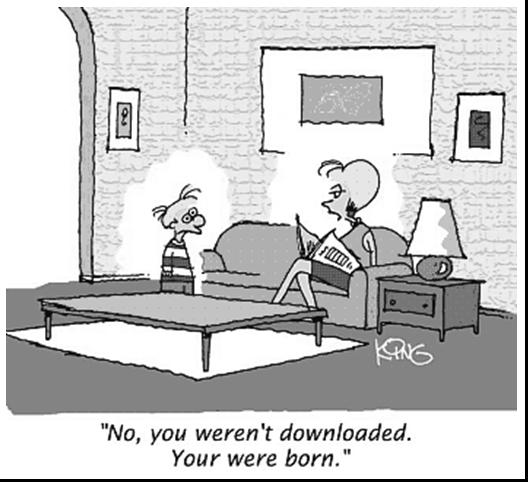
\includegraphics[width=.5\textwidth]{fig1.jpg}
\caption{A typical figure}
\label{fig:exampleFig1}
\end{figure}

\begin{figure}[ht]
\centering
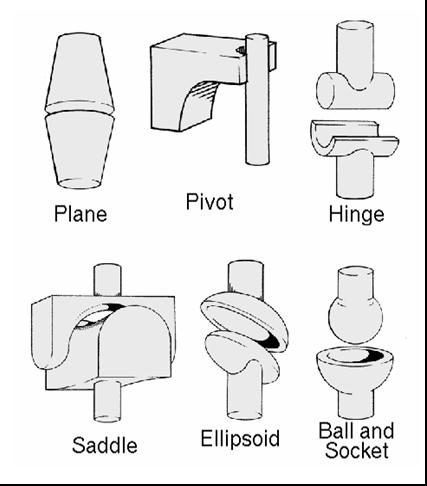
\includegraphics[width=.3\textwidth]{fig2.jpg}
\caption{This figure is an example of a figure caption taking more than one
  line and justified considering margins mentioned in Section~\ref{sec:figs}.}
\label{fig:exampleFig2}
\end{figure}

In tables, try to avoid the use of colored or shaded backgrounds, and avoid
thick, doubled, or unnecessary framing lines. When reporting empirical data,
do not use more decimal digits than warranted by their precision and
reproducibility. Table caption must be placed before the table (see Table 1)
and the font used must also be Helvetica, 10 point, boldface, with 6 points of
space before and after each caption.

\begin{table}[ht]
\centering
\caption{Variables to be considered on the evaluation of interaction
  techniques}
\label{tab:exTable1}
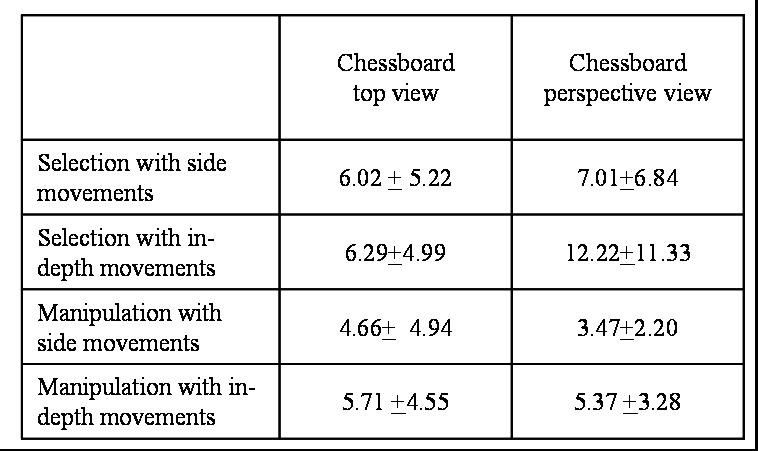
\includegraphics[width=.7\textwidth]{table.jpg}
\end{table}

\section{Images}

All images and illustrations should be in black-and-white, or gray tones,
excepting for the papers that will be electronically available (on CD-ROMs,
internet, etc.). The image resolution on paper should be about 600 dpi for
black-and-white images, and 150-300 dpi for grayscale images.  Do not include
images with excessive resolution, as they may take hours to print, without any
visible difference in the result. 

\section{References}

Bibliographic references must be unambiguous and uniform.  We recommend giving
the author names references in brackets, e.g. \cite{knuth:84},
\cite{boulic:91}, \cite{smith:99}, and \cite{alfio:14}.

The references must be listed using 12 point font size, with 6 points of space
before each reference. The first line of each reference should not be
indented, while the subsequent should be indented by 0.5 cm.

\bibliographystyle{sbc}
\bibliography{sbc-template}

\end{document}
